\section{System Overview}
Task 1: The system is mainly divided into 2 Components: The ESP32 and also a Computer as host(broker). The ESP32 is the publisher and subscriber, which sends RSS information and also receive UI command from the host. For the computer, it acts as a broker that hosts the server and collects the RSS information using MQTT. In addition, a client is also subscribe to the published rss data using rss/data. The client then collects the SSID, MAC Address and RSSI value for further processing (Localization algorithm). Details of each component will be illustrated below.

ESP32: (main.cpp)
The ESP32 is first configured using Platformio via VS Code. Through main.cpp, the ESP then prints all received signals, including SSID, MAC Address and also RSSI signal. After collection of the RSS data, the ESP32 establishes connection and sends the data to the broker and listeners through MQTT. 

Laptop (Broker): (main.py)
The broker is hosted on the laptop, in the case of macOS, host the broker using command "brew services start mosquitto". And then, python client is used to listen to the RSS data sent from ESP32. 

\section{Algorithm Design}
Full code in task 3.py 
For the algorithm design, we decided to use the method of ranging based localization, which employs a path loss model in order to perform a more accurate localization algorithm compared to Max RSSI based localization and weighted centroid. 

The localization algorithm used in the code is a two-step process involving RSSI-to-distance conversion and position estimation. 

RSSI-to-Distance Conversion (task3localization function): This function takes in RSSI values, access point (AP) locations, a path loss exponent n, and the RSSI value at 1 meter A. The path loss exponent si summarized from findings on websites, while the A variable is collected from our own experiment. In order to get a more accurate path loss exponent, we did a linear regression model (Please refer to the plot function in task4.py. It first converts the RSSI values to distances using the formula for the Log-distance path loss model. If any of the calculated distances are not valid (NaN or infinity), it returns None. Otherwise, it proceeds to the next step.

Position Estimation (estimateposition function): This function estimates the position of the device based on the distances to the APs and their locations using triteration. It defines an error function that calculates the sum of the squared differences between the actual distances to the APs and the distances calculated from the estimated location x. It then uses the minimize function from the scipy.optimize module to find the location x that minimizes this error. The minimize function uses the Nelder-Mead method, which is a numerical optimization algorithm for finding the minimum of a function in a multidimensional space.

In summary, the algorithm first converts the RSSI values to distances, then uses these distances and the known AP locations to estimate the position of the device.



\section{Evaluation}
Full code in task 4.py
The evaluation of the localization algorithm is in task4.py. First, we open the both pickle files and loops through the rssi values and runs the algorithms. With the results of the algorithm, it is then compared with the actual ground truth (label) for checking of error using Euclidean distance as the error metric. The mean, median error of each data set is returned, along with a figure of cumulative distribution figure. \\

Data Set 1 Mean error: 3.262207885146745\\
Data Set 1 Median error: 3.0838904633112056\\
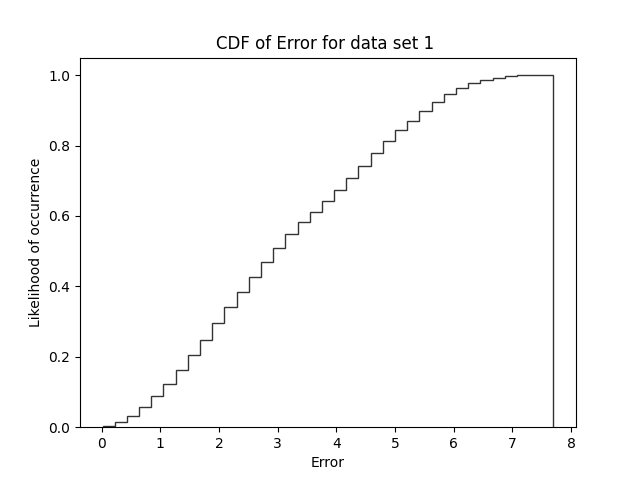
\includegraphics[width=0.4\textwidth]{error_cdf1.png}\\

Data Set 2 Mean error: 5.241855904005981 \\
Data Set 2 Median error: 5.446157651902656\\ 
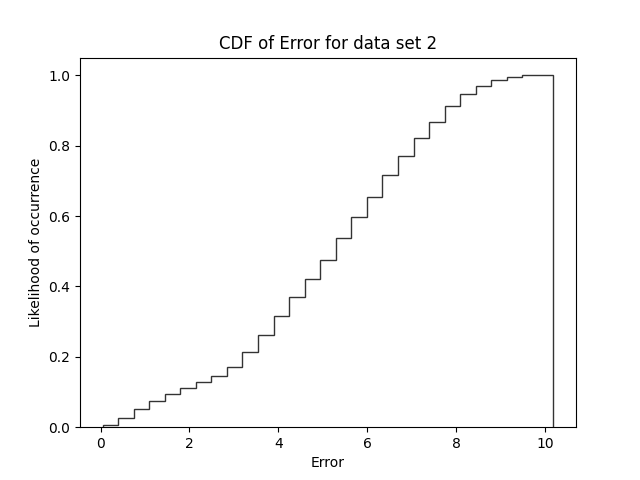
\includegraphics[width=0.4\textwidth]{error_cdf2.png}\\

\section{Real-world Experiments}

\subsection{War-Driving}
By performing RSSI observations using our system, we have successfully found out 5 AP in Chi Wah learning commons. Their SSID (AP name) are all "HKU"\\
We use  RSSI trace below to determine the AP locations:\\
\\
{"wyk21-46:E1:2F:13:6B:11": ["-36", "-32", "-42", "-39", "-40", "-37", "-40", "-40", "-30", "-24", "-22", "-22", "-25", "-26", "-23", "-22", "-22", "-25", "-23", "-21", "-21", "-26", "-25", "-33", "-41", "-26", "-37", "-34", "-38", "-28", "-41", "-32", "-26", "-30", "-31", "-27", "-35", "-25", "-33", "-39", "-31", "-34", "-31", "-36", "-38", "-33", "-39", "-35", "-36", "-30", "-43", "-12", "-8", "-14"], "HKU-30:C5:0F:68:8B:E0": ["-48", "-54"], "HKU-30:C5:0F:68:8A:E0": ["-54"], "HKU-30:C5:0F:68:8D:20": ["-54", "-56", "-45", "-39", "-44", "-48", "-54"], "HKU-30:C5:0F:68:8D:60": ["-41", "-39", "-42", "-43"], "HKU-30:C5:0F:68:92:A0": ["-49", "-48", "-51", "-46", "-43", "-43", "-52", "-45", "-43", "-51", "-58"], "HKU-30:C5:0F:68:90:A0": ["-43", "-44", "-47", "-45"], "HKU-30:C5:0F:68:93:20": ["-46", "-46", "-41", "-40", "-45", "-46", "-46", "-37", "-42"], "HKU-30:C5:0F:68:97:60": ["-50", "-48", "-47", "-38", "-47", "-39", "-35", "-42", "-44"], "HKU-30:C5:0F:68:84:20": ["-42"]}\\
\\
The wyk21 is the host wifi for mqtt, so we can neglect it. While we performing RSSI observation, we were walk around. When we constantly receive RSSI of a AP below 50, we can assume a AP is nearby\\


1: MAC: 30:C5:0F:68:8B:E0 In front of Quiet study room\\
2: MAC: 30:C5:0F:68:8D:20 Next to the service counter\\
3: MAC: 30:C5:0F:68:93:20 In front of the staircase\\
4: MAC: 30:C5:0F:68:92:A0 Between the staircase and the exit gate\\
5: MAC: 30:C5:0F:68:97:60 Close to the exit gate\\
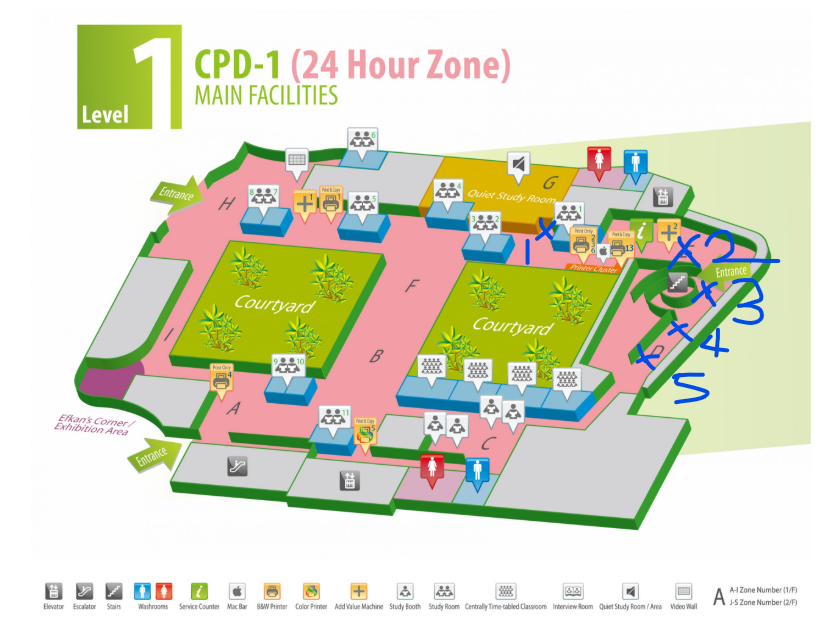
\includegraphics[width=0.4\textwidth]{Markedfloorplan.png}\\

% add whatever you want

\section{Contribution Statement}
Lam Pak Hei Jason:\\
Setup of ESP32, RSSI data collcection, Localization algorithm, evaluation of algorithm\\ 
Ng Ching Ngai:\\
War-Driving Experiment, Setup of ESP32\\

Chan Ka Ho: \\
War-Driving Experiment, algorithm optimization and evaluation 

Wong Yan Kit: \\
ESP 32 setup, Mqtt setup, War-Driving experiment
